\chapter{Troubleshooting}

\section{Introduction}

This chapter contains proposed solutions to some of the problems that was encountered over the course of the semester. The solutions are not complete or comprehensive, but may provide some quick fixes for any students that may continue working with this project.

\section{Hardware}

\subsection{The Wheel Fell Off!}

During a test drive with the robot, the base collapsed because one of the wheel shafts had slipped out of the motor drive shaft. The solution to the problem is simply to tighten the set screw which connects the motor shaft to the wheel. The set screw is shown in figure \ref{fig:set_screw}.

\begin{figure}[h]
	\centering
	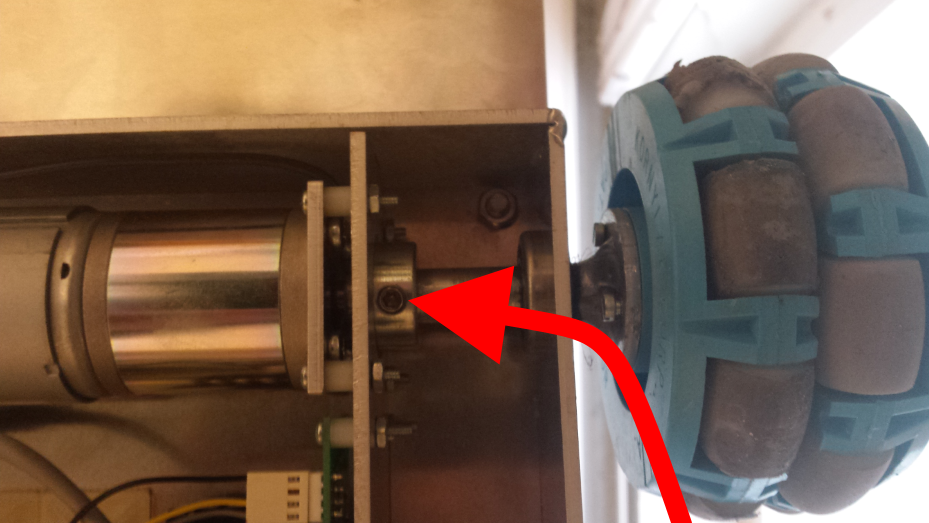
\includegraphics[width=0.8\textwidth]{set_screw}
	\caption{The set screw which holds the wheel onto the motor drive shaft.}
	\label{fig:set_screw}
\end{figure}

\section{ROS}

\subsection{\textcolor{red}{ERROR:} tf2:ExtrapolationException}
\label{sec:tfException}
When running the released ROS distribution binary of \texttt{RTAB-Map} installed with \texttt{apt-get} on the robot, the node would crash after a few iterations. The error message is as follows:

\begin{verbatim}
	Lookup would require extrapolation into the future, ..., when looking 
	up transform from frame [laser] to frame [base_link].
\end{verbatim}

The requested transform is milliseconds ahead of ''now''. This issue was fixed by maintainers in March 2016\footnote{\url{https://github.com/introlab/rtabmap_ros/issues/54}}, but was not yet integrated into the released binary. During work with this project, the problem was solved by building \texttt{RTAB-Map} from source, where the most recent fixes are included. This is a straight forward procedure, which is described on the project's GitHub repository. 

\section{Gazebo}

\subsection{\textcolor{red}{Error [Node.cc.90]} No namespace found}

\textbf{Solution: } Remember to source the \textit{gazebo} installation. In this case, with \textit{gazebo-2.2} installed as recommended for \ac{ROS} Indigo, the setup file can be sourced by typing

\begin{verbatim}
	$ source /usr/share/gazebo-2.2/setup.sh
\end{verbatim}

\subsection{Dependency Issues When Installing \textit{gazebo2}}

This problem was encountered after removing gazebo and then typing

\begin{verbatim}
$ sudo apt-get upgrade
\end{verbatim}

When typing 

\begin{verbatim}
$ sudo apt-get install -y gazebo2
\end{verbatim}

the installation failed because some dependencies had been upgraded to an incompatible version. To solve this, take note of the missing dependencies listed after entering the command above, open Ubuntu Software Center and select the History tab. Scroll down and locate the missing dependencies. They should have a red X next to them, indicating that they have been uninstalled. Then, enter the following command:

\begin{verbatim}
$ sudo apt-get install <NAME OF THE UNINSTALLED DEPENDENCY>
\end{verbatim}

%\textit{gazebo2} 

\section{Ubuntu}

\subsection{Ubuntu Freezes}

Sometimes during work with the project, Ubuntu would freeze and become unresponsive to keyboard input and mouse clicks. The mouse could be moved around, but was otherwise unresponsive. This event occurred exclusively when using \texttt{rviz} and displaying a camera topic as an image in the lower left corner of the \ac{GUI}. The following steps from a post at \href{http://askubuntu.com/questions/4408/what-should-i-do-when-ubuntu-freezes/36717#36717}{askubuntu.com}\footnote{What to do when Ubuntu freezes: \url{http://askubuntu.com/questions/4408/what-should-i-do-when-ubuntu-freezes/36717\#36717}}, solves the problem.
%\cite{Reboot_Ubuntu}:

While holding \keystroke{Alt} and \keystroke{SysReq (Print Screen)}, type \keystroke{R}\keystroke{E}\keystroke{I}\keystroke{S}\keystroke{U}\keystroke{B}. Press each key properly, and allow a few seconds to pass between each keystroke so that each command has time to execute. This should cause the computer to reboot, and is supposedly safer than using the power button. See the footnote for more information.